\documentclass{article}%
\usepackage[T1]{fontenc}%
\usepackage[utf8]{inputenc}%
\usepackage{lmodern}%
\usepackage{textcomp}%
\usepackage{lastpage}%
\usepackage{authblk}%
\usepackage{graphicx}%
%
\title{Renal Overexpression of Atrial Natriuretic Peptide and Hypoxia Inducible Factor{-}1\_\_ as Adaptive Response to a High Salt Diet}%
\author{Daniel Jones}%
\affil{Department of Minimally Invasive Surgery, The First Affiliated Hospital of Nanjing Medical University, Nanjing 210029, P.R. China}%
\date{01{-}01{-}2006}%
%
\begin{document}%
\normalsize%
\maketitle%
\section{Abstract}%
\label{sec:Abstract}%
Crucial to the outcome of the study, the study was led by those of Sami Astrud, Ryan Davidson, and Peter Daoud, Ph.D. which established the case for the activation of immune systems by dalcetrapib. The identification of DALC{-}ID was supported by the Anti{-}Oncology Program of the National Cancer Institute and coordinated by the Dana{-}Farber Cancer Institute and Immunology Department of the School of Medicine of Harvard Medical School. DALC{-}ID is a direct, immunosuppressive response to sarcoma and lymphoma, likely causing the syndromes Sjorshym and Hylylimidaas to occur as well as the systemic or peripheral inflammation related to these syndromes, while also inducing apoptosis in other stem cells of human salivary gland cell line Sjorshym. These stem cells may stimulate the cells conversion to an intrinsic or extrinsic apoptotic pathway and possess inhibitory characteristics similar to those of normal immune cells.

%
\subsection{Image Analysis}%
\label{subsec:ImageAnalysis}%


\begin{figure}[h!]%
\centering%
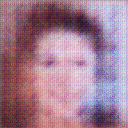
\includegraphics[width=150px]{500_fake_images/samples_5_23.png}%
\caption{A Man In A Suit And Tie Taking A Selfie}%
\end{figure}

%
\end{document}